\chapter{Versuchsvorbereitung}
Für eine zielorientierte Durchführung des Versuchs 3 in Elektronik 1 Praktikum haben wirdas Ziel definiert.
    \section{Ziele des Versuchs}
        Das Ziel in diesem Versuch ist es, die Aufnahme der Kennlinie eines NPN-Transistor vom Typ BC547 kennen zu lernen. Darüber hinaus soll man seine chrakteristischen Größen bestimmmen können.

    \section{Begriffserklärung}
        \subsection{Eingangskennlinie}
            Die \textbf{Eingangskennlinie} stellt den Zusammenhang zwischen der Basis-Emitter-Spannung \(U_{BE}\) und dem Basisstrom \(I_B\) dar. Sie entspricht auch der Kennlinie einer Diode.
        \subsection{Stromsteuerkennlinie}
            Die \textbf{Stromsteuerkennlinie} beschriebt die Abhängigkeit des Kollektorstroms \(I_C\) vom Basisstrom \(I_B\). 
        \subsection{Ausgangskennlinienschar}
            Der Basisstrom regelt den Strom \(I_C\) im Hauptstromkreis zwischen Kollektor und Emitter. Außerdem spielt die Spannung zwischen diesen zwei kaum eine Rolle. Der Transistor verhält sich an der Ausgangsseite wie eine Stromquelle. So mit der der Kollektor-Emitterwiderstand abhängig von der Spannung.
        \subsection{differentieller Eingangswiderstand}
            Durch den nicht linearen Kurvenverlauf ist der Eingangsleitwert immer unterschiedlich und abhänging von der Ansteuerung. Die Steigung eines auf der Kurve liegender Arbeitspunkt kann durch seine Tangente ermittelt werden. Aus seinem Kehrwert errechnet sich dann der \textbf{differentieller Eingangswiderstand}. 
            Der Wert des Widerstands ändersich wenn die Spannung \(U_{CE}\) nicht konstant ist.
            Im Standard fall bei Transistoren liegt dieser Bereich zwischen 100 \(\Omega \) bis 50 \(k\Omega \). [Quelle: https://www.elektroniktutor.de/bauteilkunde/transkl.html 08.01.2021]
        \subsection{differentieller Ausgangswiderstand}
            Wie bei dem differentiellen Eingangswiderstand steht der \textbf{differentieller Ausgangswiderstand} auch für den Anstieg an einem bestimmmen Punkt in der Kennlinie.
            Dieser Widerstand ändert sich wenn der Strom \(I_B\) nicht konstant ist auf einen bestimmten Arbeitspunkt bezogen.

    \section{Versuchsaufbau}
        Um den Versuch durchführen zu können wird eine Schaltung verwendet die man auch im Skript von Herrn Dörr aus Elektronik 1 finden ist (Seite 79). 
         \begin{figure}[h!]
            \centering
            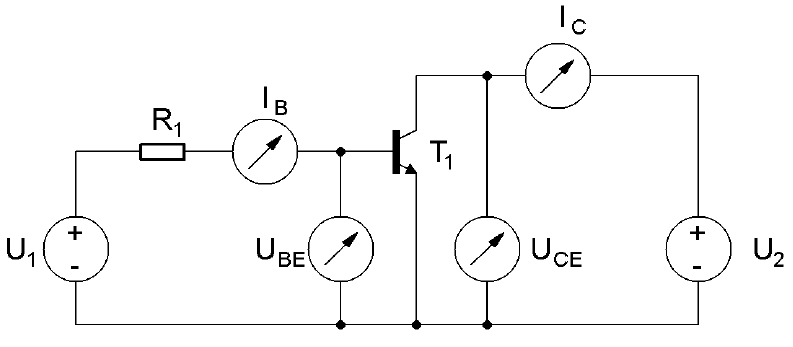
\includegraphics[width=9cm]{Bilder/npn_transistorschaltung.PNG}
            \caption{Schaltung zur Aufnahme der Kennlinien eines NPN-Transistor}
            \label{fig:npn_transistor}
         \end{figure}